\chapter{Vývoj zařízení - Řídící software}
\label{5-vyvoj-zarizeni-ridici-software}
%V této kapitole bude popsána tvorba řídícího programu pro Arduino.

\section{Programovací jazyk}

Nejběžněji bývá pro tvorbu řídícího programu pro Arduino využívána varianta jazyka C++, která využívá struktury převzaté z~jazyka Wiring. Alternativně lze použít jazyky jako MicroPython, JavaScript a další. Ve Wiringu se namísto typické funkce \texttt{main} pro C++ používají funkce \texttt{setup} pro prvotní inicializaci při spuštění programu a funkce \texttt{loop} pro nekonečnou smyčku, která program nepřetržitě vykonává \cite{arduino}.

\section{Vývojové prostředí}
Pro tvorbu a nahrání řídicího programu do mikrokontroléru se využívá \zkratka{IDE}. Mikrokontroléry, na rozdíl od jednodeskových mikropočítačů, nejsou vybaveny operačním systémem. Nelze tedy tvořit kód přímo na mikro\-kontroléru, je potřeba jej vytvořit na počítači, zkompilovat a následně nahrát jako binární soubor do mikro\-kontroléru. Pro tvorbu řídicího programu bylo konkrétně využito Arduino \zk{IDE}. To nabízí kromě možnosti psaní, kompilování a nahrávání kódu i správu knihoven a čtení dat z~Arduina pro ladění kódu. Kromě vývojového prostředí Arduino \zk{IDE} bylo využíváno prostředí VS Code od společnosti Microsoft, které umožňuje verzování pomocí Gitu a sdílení kódu na platformě GitHub.

\begin{figure}[H]
	\centering
	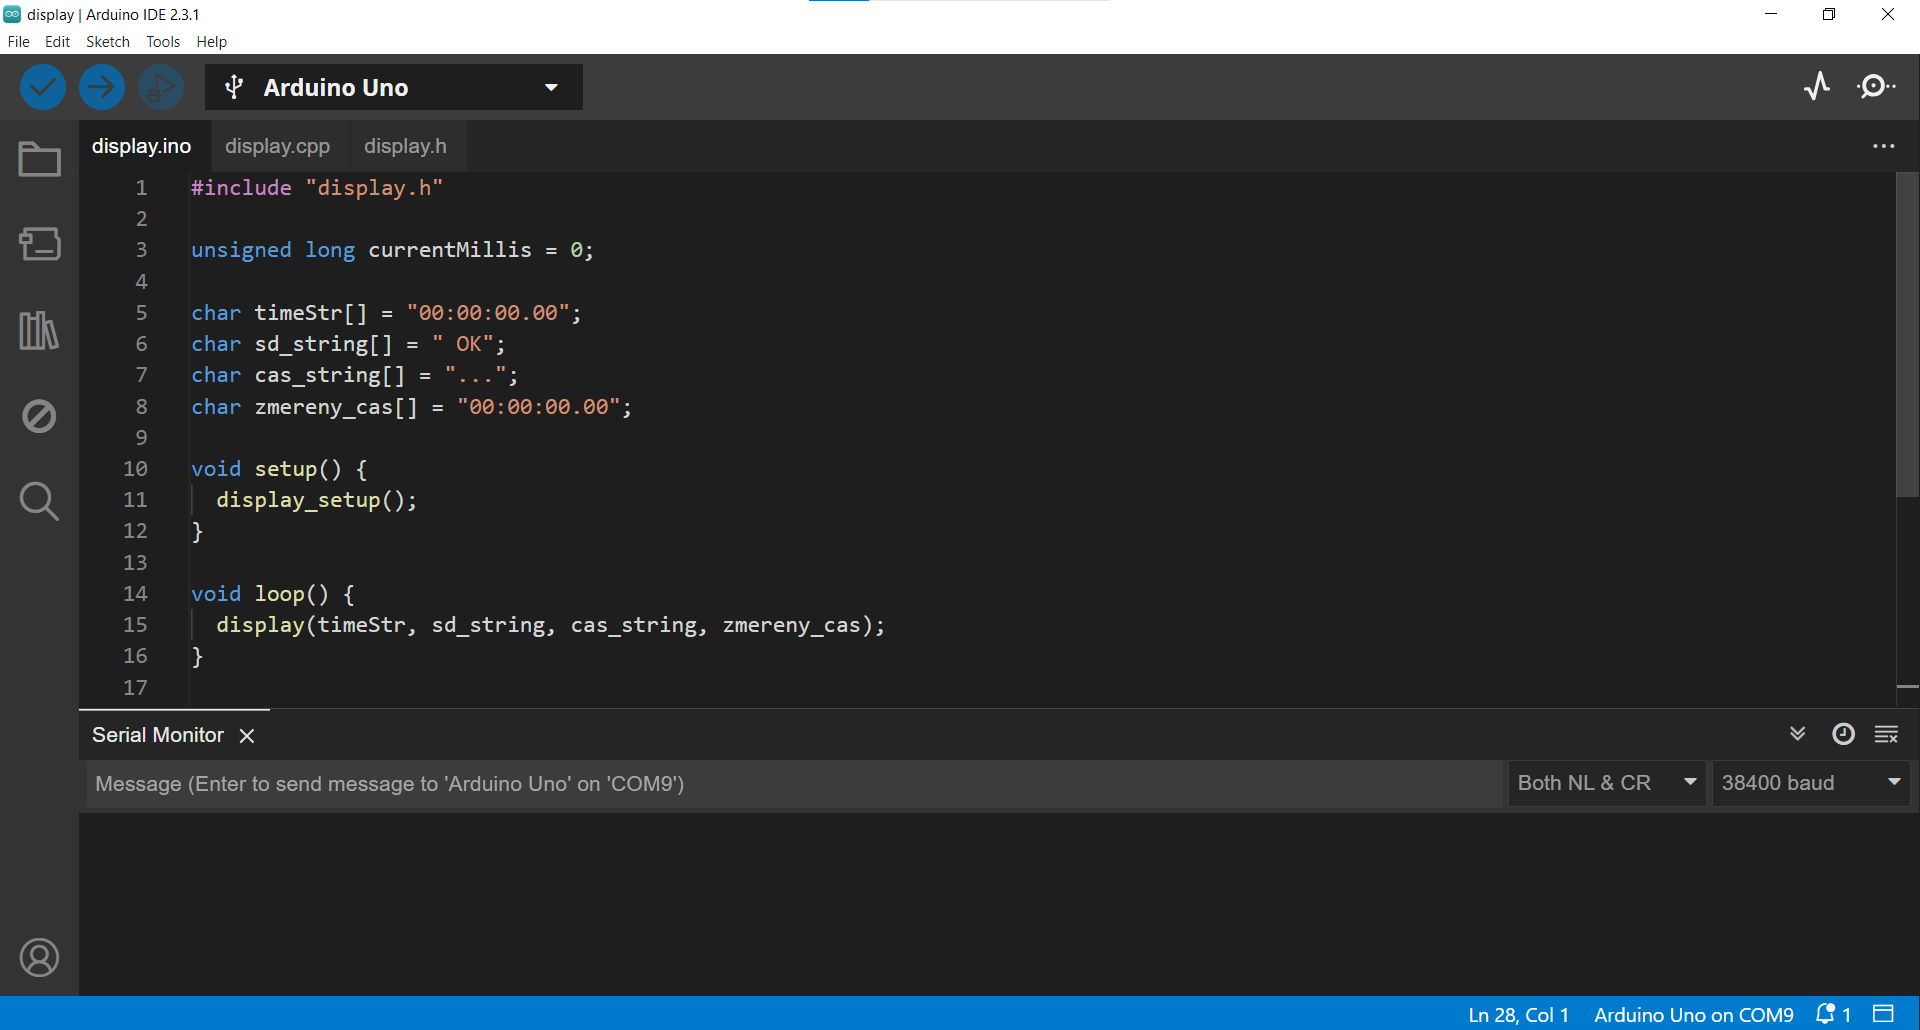
\includegraphics[width=14.5cm]{images/komponenty/Arduino_IDE.png}
	\caption{Arduino IDE}
\end{figure}

\section{Použité knihovny}
Pro práci s~některými komponenty byly využity již existující knihovny, které usnadňují využití jejich funkcionality. Knihovna \href{https://www.arduino.cc/en/Reference/SoftwareSerial}{\texttt{SoftwareSerial.h}} byla využita pro emulaci pinů sloužících pro sériovou komunikaci, protože Arduino UNO obsahuje pouze jeden TX a jeden RX pin, určený pro sériovou komunikaci. Pro práci s~údaji o~čase byla využita knihovna \href{https://www.pjrc.com/teensy/td_libs_Time.html}{\texttt{TimeLib.h}}. Pro synchronizaci času prostřednictvím signálu z~DCF77 přijímače byla využita knihovna \href{https://github.com/thijse/Arduino-DCF77}{\texttt{DCF77.h}}. Tato knihovna obsahuje funkce pro dekódování signálu DCF77. Pro přístup k~NTP serveru byly využity knihovny \href{https://github.com/esp8266/Arduino/tree/master/libraries/ESP8266WiFi}{\texttt{WiFiS3.h}} a \href{https://www.arduino.cc/en/Reference/WiFi}{\texttt{WiFiUdp.h}}. Ty slouží pro připojení k~WiFi a přijímaní a odesílání paketů, které využívá NTP server. Pro práci s~Micro SD kartou byla využita knihovna \href{https://www.arduino.cc/en/Reference/SD}{\texttt{SD.h}}. Tato knihovna obsahuje funkce pro zapisování dat na Micro SD kartu a čtení dat z~ní. Pro práci s~OLED displejem byla nejprve využívána knihovna \href{https://github.com/olikraus/u8glib}{\texttt{U8glib.h}}, která ale není kompatibilní s~mikrokontroléry Renesas, a tak byla využita knihovna \href{https://github.com/olikraus/u8g2}{\texttt{U8g2lib.h}}. Pro práci s~hlasovým modulem byla využita knihovna \href{https://github.com/DFRobot/DFRobotDFPlayerMini}{\texttt{DFRobotDFPlayerMini.h}}.

\section{Členění kódu}
Řídící program byl rozdělen z~důvodu přehlednosti na hlavní program \texttt{(*.ino)}, který sdružuje další části kódu ve formě hlavičkových (\texttt{*.h}) a implementačních souborů (\texttt{*.cpp}). Během tvorby řídícího programu byly využity již existující kniho\-vny a při tvorbě kódu bylo vycházeno ze vzorových kódů, které k~nim byly přiložené v~dokumentaci. Nicméně některé části kódu byly vytvořeny zcela nově. \text{Například} bylo potřeba zajistit, aby stisknutí tlačítka bylo považováno za stisknutí pouze v~prvním průchodu funkcí \texttt{loop}, a v~dalších průchodech již nebylo tlačítko považováno za stisknuté tak, aby bylo provedeno při každém stisku jen jedno měření a měření bylo přehledné a jednoznačné. Kód pro příjem dat z~GNSS přijímače byl vytvořen také kompletně od začátku. V~tomto kódu je načítána pomocí sériové komunikace NMEA zpráva. Ta je parsována a je z~ní zjišťováno, zda byla určena poloha přijímače. Pokud je určena poloha přijímače lze považovat čas za aktuální. V~tom případě je text s~časem převeden na číselné hodnoty a s~těmi je dále praco\-váno. Dalším pří\-kladem je funkce setiny. Jelikož všechny použité přijímače poskytují data po celých sekundách, tak byla vytvořena funkce setiny, která je spuštěna vždy na začátku celé sekundy a rozděluje ji na setiny sekund. Při každé nové sekundě jsou setiny sekund vynulovány. Od začátku byla také vyhotovena část kódu pro komunikaci s~totální stanicí a další části kódu.

\vspace{1cm}

\begin{figure}[H]
\hspace{-1cm}
\begin{tikzpicture}[
    startstop/.style={rectangle, rounded corners, minimum width=2cm, minimum height=0.5cm,text centered, draw=black, fill=red!30},
    io/.style={trapezium, trapezium left angle=70, trapezium right angle=110, minimum width=2cm, minimum height=0.5cm, text centered, draw=black, fill=blue!30},
    process/.style={rectangle, minimum width=2cm, minimum height=0.5cm, text centered, draw=black, fill=orange!30},
    decision/.style={diamond, minimum width=2cm, minimum height=0.5cm, text centered, draw=black, fill=green!30},
    arrow/.style={thick,->,>=stealth},
]

\node (init) [startstop] {Inicializace zařízení};
\node (sdCheck) [process, below of=init, yshift=-0.25cm] {Kontrola připojení micro SD karty};
\node (timeAttempt) [process, below of=sdCheck, yshift=-0.25cm] {Pokus o~aktualizaci času};
\node (display) [process, below of=timeAttempt, yshift=-0.25cm] {Zobrazení aktuálního stavu na displeji};
\node (buttonCheck) [decision, below of=display, yshift=-2cm, align=center] {Kontrola\\stisknutí\\tlačítka};
\node (saveTime) [process, right of=buttonCheck, xshift=5.5cm] {Uložení aktuálního času};
\node (tsRequest) [process, below of=saveTime, yshift=-0.25cm] {Odeslání požadavku TS};
\node (saveTsData) [process, below of=tsRequest, yshift=-0.25cm] {Uložení dat z~TS};
\node (info) [process, below of=saveTsData, yshift=-0.25cm] {Signalizace};
\node (btCheck) [decision, below of=buttonCheck, yshift=-3.75cm, align=center] 
{Kontrola\\ požadavku\\ Bluetooth};

\node (uzel) [startstop, left of=btCheck, xshift=-5cm, align=center, fill=white, draw=white] {};

\node (openFile) [process, below of=btCheck, yshift=-2.1cm] {Otevření souboru s~měřenými daty};
\node (sendData) [process, below of=openFile, yshift=-0.25cm] {Odeslání dat přes Bluetooth};

\draw [arrow] (init) -- (sdCheck);
\draw [arrow] (sdCheck) -- (timeAttempt);
\draw [arrow] (timeAttempt) -- (display);
\draw [arrow] (display) -- (buttonCheck);
\draw [arrow] (buttonCheck.east) -- ++(1,0) |- node[yshift=0.2cm] {ano} (saveTime.west);
\draw [arrow] (saveTime) -- (tsRequest);
\draw [arrow] (tsRequest) -- (saveTsData);
\draw [arrow] (saveTsData) -- (info);
\draw [arrow] (info) |- (btCheck);

\draw [arrow] (btCheck.west) -- ++(0,0) |- node[yshift=0.2cm,xshift=-2cm] {ne} (uzel.center);

\draw [arrow] (buttonCheck) -- node[anchor=east] {ne} (btCheck);
\draw [arrow] (btCheck) -- node[xshift=0.5cm] {ano} (openFile);
\draw [arrow] (openFile) -- (sendData);
\draw [arrow] (sendData) |- ++(0,-1) -- ++(-6,0) |- (sdCheck);

\end{tikzpicture}
\caption{Zjednodušené schéma řídícího programu}
\end{figure}




% https://bastlirna.hwkitchen.cz/zakladni-struktury-jazyka-wiring/

% https://www.arduino.cc/reference/en/